\documentclass[11pt,a4paper]{article}
\usepackage[a4paper,hmargin=1in,vmargin=1in]{geometry}
\usepackage{pgfplots}
\pgfplotsset{compat=1.17}

\usepackage[czech]{babel}
\usepackage[utf8]{inputenc}
\usepackage[T1]{fontenc}

\usepackage{stddoc}




\begin{document}
\pagenumbering{arabic}


% Needlessly fancy header
    \begin{center}
        \section*{Osnova k výuce přípravných kurzů fyziky}
        \vspace*{-4mm}
        \begin{minipage}{0.4\textwidth}
            \begin{flushleft}
                \textsc{\today}
            \end{flushleft}
        \end{minipage}
        ~
        \begin{minipage}{0.4\textwidth}
            \begin{flushright}
                \textsc{Martin Šimák}
            \end{flushright}
        \end{minipage}
        \noindent\rule{14.5cm}{0.6pt}
    \end{center}


% First lecture
    \section*{Přednáška první}

        \subsection*{Kinematika}

            \begin{itemize}
                \item Pojem poloha - funkce času $x(t)$, nakreslit obecný graf pohybu hmotného bodu v 1D.
                \item Rychlost $v(t)$ a zrychlení $a(t)$. Obecně se taky mohou měnit s časem - taktéž funkce času.
            \end{itemize}
            \paragraph*{Příklady.}
            \begin{enumerate}
                \item Bod A má souřadnici $x_A = 2$ m a bod B je od něj vzdálen 3 metry. Jakou má souřadnici bod B? [$x_B \in \{-1 \;\mathrm m, 5 \;\mathrm m\}$]. Nakreslit.
                \item Přesun do 2D: Body A a B mají souřadnice $\vec r_A = (1,1)^{\mathrm T}$ m a $\vec r_B = (4,-3)^{\mathrm T}$ m. Jaká je jejich vzájemná vzdálenost?
                \begin{align*}
                    \norm{\vec r_A - \vec r_B} = \norm{(-3,4)^{\mathrm T}} = \sqrt{9 + 16} = 5.
                \end{align*}
                
                \item Jaké má souřadnice bod B, jestliže bod A má souřadnice $(1,2)$ a jejich vzájemná vzdálenost je 3? Nekonečno řešení, museli bychom zadat vektor vzájemné vzdálenosti pro jednoznačnost.
            \end{enumerate}

            \begin{itemize}
                \item Rovnoměrný pohyb: zrychlení $a(t) = 0$, tj. $v(t) = s/t \in \R$ (konstanta). Můžeme potom psát, že okamžitá poloha je $x(t) = x_0 + vt$ pro $t_0 = 0$, jinak $x(t) = x_0 + v(t-t_0)$, kde $x_0 = x(t_0)$, a dráha $s(t) = vt$.
                \item Vysvětlit rozdíl mezi $s$ a $x$. Poloha $x(t) = x_0 + vt$, kdežto dráha $s(t) = vt$ jakožto vzájemná vzdálenost dvou bodů.
                \item Pro rovnoměrný pohyb je okamžitá rychlost v každém čase rovna průměrné rychlosti na libovolném časovém úseku.
                \begin{align*}
                    \bar v(t) = \frac{\Delta x(t)}{\Delta t} = \frac{\Delta s(t)}{\Delta t}.
                \end{align*}
            \end{itemize}
            \paragraph*{Příklady.}
            \begin{enumerate}
                \item Pepa jede za Karlem z Prahy do Brna (vzdálenost $s = 200$ km), což mu zabere zhruba $t = 2$ h. Jakou rychlostí (za předpokladu pohybu rovnoměrného) Pepa jel?
                \begin{align*}
                    v = \frac st = \frac{200 \; \mathrm{km}}{2 \; \mathrm{h}} = 100 \; \frac{\mathrm{km}}{\mathrm h} = 100 \cdot \frac{1000}{3600} \; \frac{\mathrm{m}}{\mathrm s} = \frac{100}{3,6} \; \frac{\mathrm{m}}{\mathrm s} \approx 28 \; \frac{\mathrm{m}}{\mathrm s}.
                \end{align*}

                \item Hmotný bod se souřadnicí $x_0 = 2$ m se pohybuje konstantní rychlostí $v = 3$ m/s. Jaká bude jeho souřadnice za 4 s. [$x(t=4 \; \mathrm s) = x_0 + 4v = 2 + 4 \cdot 3 \; \mathrm m = 14 \; \mathrm m$]
                \item Obdoba ve 2D: Chodec nacházející se v čase $t_0 = 0$ s v bodě $\vec r_0 = (-1,0)^{\mathrm T}$ m jde rychlostí $v = 2$ m/s ve směru vektoru $\vec e_v = (0,1)^{\mathrm T}$. Jaká bude jeho poloha za 3 s?
                \begin{align*}
                    \vec r(t=3 \; \mathrm s) = \vec r_0 + 3 \vec v = \vec r_0 + 3v \vec e_v = \vektor{-1 \\ 0} + 6 \vektor{0\\1} \; \mathrm m = \vektor{-1 + 6 \cdot 0 \\ 0 + 6 \cdot 1} \; \mathrm m = \vektor{-1 \\ 6} \; \mathrm m.
                \end{align*}
            \end{enumerate}
            
            \begin{itemize}
                \item Rovnoměrný pohyb po kružnici o poloměru $R$: úhlová rychlost $\omega = \varphi/t = 2\pi/T$, perioda~$T$, frekvence $f=1/T$, obvodová rychlost $v = 2\pi R/T = R \omega$.
            \end{itemize}

            \begin{itemize}
                \item Rovnoměrně zrychlený pohyb: zrychlení $a(t) = v/t \in \R$ (konstanta). Potom pro rychlost platí $v(t) = v_0 + at$, pro polohu $x(t) = x_0 + v_0t + 1/2 at^2$, pro dráhu $s(t) = v_0t + 1/2 at^2$.
                \item Pro rovnoměrně zrychlený pohyb je okamžité zrychlení v každém čase rovno průměrnému zrychlení na libovolném časovém úseku.
                \begin{align*}
                    \bar a(t) = \frac{\Delta v(t)}{\Delta t}.
                \end{align*}
            \end{itemize}
            \paragraph*{Příklady.}
            \begin{enumerate}
                \item Auto dokáže zrychlit za rovnoměrného zrychlení z 0 km/h na 100 km/h za 5 s. Jakou dráhu za tuto dobu urazí?
                \begin{align*}
                    a(t) &= \frac{v_1 - v_0}{t} = \frac{v_1}{t},
                \\
                    s(t) &= v_0 t + \frac 12 a t^2 = 0 + \frac 12 \frac{v_1}{t} t^2 = \frac 12 v_1 t = 70 \; \mathrm m, \quad v \approx 28 \; \frac{\mathrm m}{\mathrm s}, \, t = 5 \; \mathrm s.
                \end{align*}
                
                \item Auto zastaví z rychlosti 64,8 km/h rovnoměrně zrychleným (zpomaleným) pohybem za 9 sekund. Spočítejte dráhu uraženou za tuto dobu.
                \begin{align*}
                    a(t) &= \frac{v_1 - v_0}{t} = - \frac{v_0}{t},
                \\
                    s(t) &= v_0t + \frac 12 a t^2 = v_0t - \frac 12 v_0 t = \frac 12 v_0 t = \frac 12 \frac{64,8}{3,6} 9 \; \mathrm m = 81 \; \mathrm m.
                \end{align*}

                \item Dvě auta jedou ze stejného místa týmž směrem. První z klidu se zrychlením o velikosti 3 ms$^{-2}$. Druhé rovnoměrným pohybem rychlostí o velikosti 54 km/h. Za jak dlouho a v jaké vzdálenosti od startu (místo startu nepočítáme) se auta setkají?
                \begin{align*}
                    s_1(t) &= v_{0,1} t + \frac 12 a_1 t^2 = \frac 12 a_1 t^2,
                \\
                    s_2(t) &= v_{0,2} t + \frac 12 a_2 t^2 = v_{0,2} t,
                \end{align*}
                První dožene v čase $t_k$ druhé:
                \begin{align*}
                    s_1(t_k) &= s_2(t_k),
                \\
                    \frac 12 a_1 t_k^2 &= v_{0,2} t_k,
                \\
                    a_1 t_k^2 - 2 v_{0,2} t_k &= 0, \quad v_{0,2} = \frac{54}{3,6} \; \mathrm m / \mathrm s = 15 \; \mathrm m / \mathrm s,
                \\
                    t_k(3 t_k - 30) &= 0, \quad t_k \neq 0,
                \\
                    t_k &= 10 \; \mathrm s.
                \end{align*}
                Uraženou dráha za čas $t_k$:
                \begin{align*}
                    s(t_k) &= s_1(t_k) = v_{0,2} t_k = 15 \cdot 10 \; \mathrm m = 150 \; \mathrm m.
                \\
                    & = s_2(t_k) = \frac 12 a_1 t_k^2 = \frac 12 \cdot 3 \cdot 10^2 \; \mathrm m = 150 \; \mathrm m.
                \end{align*}

                \item Těleso snížilo rovnoměrně zrychleným přímočarým pohybem svoji rychlost ze 72 km/h na 18 km/h za 10 s. Jakou dráhu urazilo?
                \begin{align*}
                    v_1 &= \frac{72}{3,6} \; \mathrm m / \mathrm s = 20 \; \mathrm m / \mathrm s,
                \\
                    v_2 &= \frac{18}{3,6} \; \mathrm m / \mathrm s = 5 \; \mathrm m / \mathrm s,
                \\
                    s &= v_0 t + \frac 12 at^2 = v_0 t + \frac 12 (v_1-v_0) t = 20 \cdot 10 \; \mathrm m - \frac 12 \cdot 15 \cdot 10 \; \mathrm m = 125 \; \mathrm m.
                \end{align*}

                \item Výpravčí stojí na peróně na začátku prvního vagónu stojícího vlaku. Vlak se dá do rovnoměrně zrychleného pohybu takovým způsobem, že první vagón míjí výpravčího po dobu $\Delta t_1$. Jakou dobu $\Delta t_n$ míjí výpravčího $n$-tý vagón?\\
                Označme délku vagónu $\l$ a celkový uplynulý čas při míjení výpravčího $n$-tým vagónem $t_n$. Potom
                \begin{align*}
                    \l &= \frac 12 a \Delta t_1^2,
                \\
                    n\l = \frac 12 a t_n^2 \implies t_n &= \sqrt{\frac{2n\l}{a}} = \sqrt{\frac{2n a\Delta t_1^2}{2a}} = \Delta t_1 \sqrt n,
                \\
                    \Delta t_n &= t_n - t_{n-1} = \Delta t_1 \( \sqrt n - \sqrt{n-1} \).
                \end{align*}

            \end{enumerate}

            \begin{figure}[h!]
                \centering
                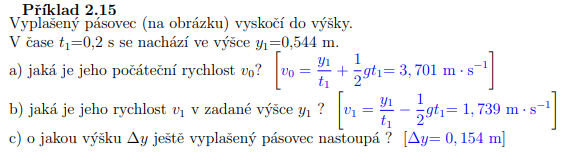
\includegraphics[width=0.9\linewidth]{figs/kin1.png}
                \caption{Příklad 6}
            \end{figure}

            \begin{figure}[h!]
                \centering
                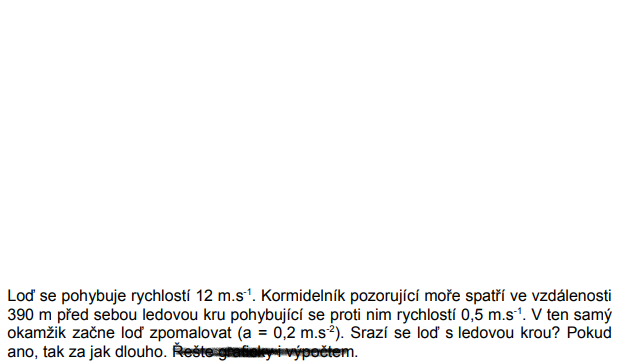
\includegraphics[width=0.9\linewidth]{figs/kin2.png}
                \caption{Příklad 7}
            \end{figure}

            \begin{figure}[h!]
                \centering
                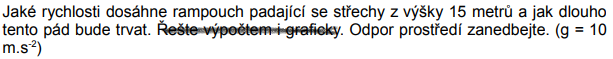
\includegraphics[width=0.9\linewidth]{figs/kin3.png}
                \caption{Příklad 8}
            \end{figure}

            \begin{figure}[h!]
                \centering
                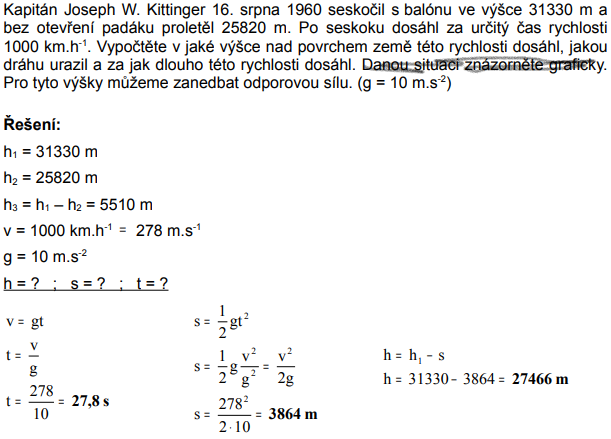
\includegraphics[width=0.9\linewidth]{figs/kin4.png}
                \caption{Příklad 9}
            \end{figure}

\newpage
    \section*{Přednáška druhá}
            
        \begin{itemize}
            \item Udělat vlak z minula a třeba ještě jeden, podle času.
            \item Jimmy mluví, já jen kreslím a mam příklady na rovnoměrný pohyb po kružnici.
        \end{itemize}
        \paragraph*{Příklady.}
        \begin{enumerate}
            \item Jakou obvodovou rychlostí se pohybuje bod na kružnici, je-li poloměr kružnice $R$ desetinásobkem periody $T$.
            \begin{align*}
                v = \frac{2 \pi R}{T} = \frac{2 \pi \cdot 10 |T|}{|T|} \; \mathrm{ms}^{-1} = 20\pi \; \mathrm{ms}^{-1}.
            \end{align*}

            \item Jaká je úhlová a obvodová rychlost otáčení Země kolem vlastní osy na rovníku? Jaké jsou tyto rychlosti pro Českou republiku? Uvažujte, že Česká republika leží na 50. stupni severní zeměpisné šířky ($\varphi = 50 \degree$).
            Poloměr Země $R_Z$ uvažujte 6400 km.
            \begin{align*}
                \omega = \frac{2\pi}{T} = \frac{2\pi}{24} \; \mathrm h^{-1} \approx 7,27 \cdot 10^{-5} \; \mathrm s^{-1}
            \end{align*}
            \begin{enumerate}[label=(\alph*)]
                \item \begin{align*}
                    R &= R_Z = 6400 \; \mathrm{km} = 6,4 \cdot 10^{6} \; \mathrm m,
                \\
                    v &= \omega R \approx 465,42 \: \mathrm{ms}^{-1}.
                \end{align*}

                \item 
                \begin{align*}
                    R &= R_Z \cos(\varphi),
                \\
                    v &= \omega R_Z \cos(\varphi) \approx 299,08 \; \mathrm{ms}^{-1}.
                \end{align*}
                \begin{figure}[h!]
                    \centering
                    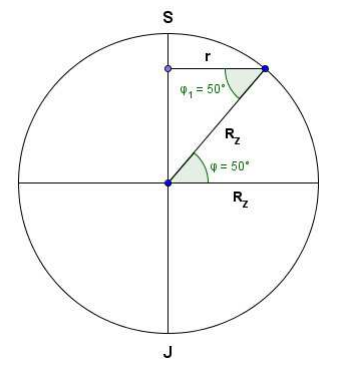
\includegraphics[width=0.4\linewidth]{figs/kin5.png}
                    \caption{Ilustrace k příkladu 2-b)}
                \end{figure}
            \end{enumerate}

            \item O kolik hertzů je frekvence bodu pohybujícího se rovnoměrným pohybem po kružnici obvodovou rychlostí $v_1 = 3 \; \mathrm{ms}^{-1}$ větší, než frekvence bodu pohybujícího se rovnoměrným pohybem po stejné kružnici obvodovou rychlostí $v_2 = 2 \; \mathrm{ms}^{-1}$. Poloměr kružnice je $R = 0,5 \; \mathrm m$.
            \begin{align*}
                v &= 2 \pi f R,
            \\
                f &= \frac{v}{2 \pi R},
            \\
                \Delta f &= f_1 - f_2 = \frac{v_1 - v_2}{2\pi R} \approx 0,32 \; \mathrm{Hz}.
            \end{align*}

            \item Náboj vystřelený z pušky letí přímým směrem rychlostí $v = 300 \; \mathrm{ms}^{-1}$ a zároveň se otáčí kolem své podélné osy úhlovou rychlostí $\omega = 0,175 \;\mathrm{rad}\cdot\mathrm{s}^{-1}$. O jaký úhel se otočí po uražení dráhy $s = 100 \;\mathrm m$? Předpokládejme, že rychlost náboje se nemění.\\
            Z definic:
            \begin{align*}
                v = \frac{s}{t}, \quad \omega = \frac{\varphi}{t},
            \end{align*}
            čas uplynul stejný, musí proto platit
            \begin{align*}
                \frac{\varphi}{\omega} &= \frac{s}{v},
            \\
                \varphi &= \omega \frac sv \approx 0,058 \approx 3,34 \degree.
            \end{align*}

            \item Automobil projíždí zatáčkou o poloměru $R = 50 \;\mathrm m$ rychlostí o stálé velikosti $ v = 36 \; \mathrm{kmh}^{-1}$. Jak velké je normálové zrychlení automobilu v zatáčce?
            \begin{align*}
                v &= 10 \; \mathrm{ms}^{-1},
            \\
                a_n &= \frac{v^2}{R} = 2 \;\mathrm{ms}^{-2}.
            \end{align*}
        \end{enumerate}
                
            

            

        

\end{document}